\documentclass[tikz]{standalone}
\usetikzlibrary{shapes.geometric}
\begin{document}
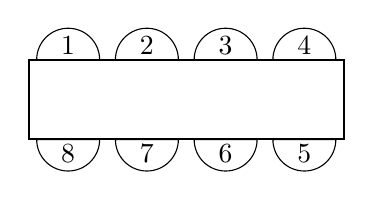
\begin{tikzpicture}[every node/.style = draw, inner sep = 2pt, semicircle]
\begin{scope}[anchor = north, shape border rotate = 180]
    \node at (0,0)  {8};
    \node at (1,0)  {7};
    \node at (2,0)  {6};
    \node at (3,0)  {5};
\end{scope}
\begin{scope}[anchor = south]
    \node at (0,1)  {1};
    \node at (1,1)  {2};
    \node at (2,1)  {3};
    \node at (3,1)  {4};
\end{scope}
\draw [thick] (-.5,0) rectangle (3.5, 1);
\end{tikzpicture}
\end{document}

